Even if you own an Arduino and have programmed it for many moons using C++ (and the Wiring libraries), we want to make sure that you're ``good to go'' when you start using \occam and the \plumbing libraries. 

\GOALS
The goals for this chapter are for you to:

\begin{enumerate}
	\item Install the FTDI drivers for the Arduino.
	\item Install our JEdit-based IDE (which will show up as the {\em Transterpreter}).
	\item See if things work.
\end{enumerate}

\section{Installing the Drivers---or Not}
This is tricky. Depending on what kind of ``Arduino'' you have, you may, or may not, need to install some drivers. This isn't special to \occam or \plumbing; the same is true if you are programming your Arduino using Wiring.

Lets look at what might be the case here:

\subsection{You have an old Arduino}
If you have an older Arduino, it might have a little chip that looks like this:

\begin{figure}[ht]
  \begin{center}
    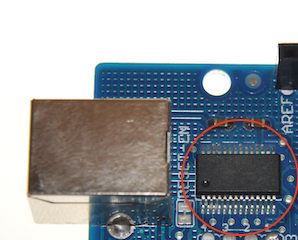
\includegraphics[width=0.8\linewidth]{images/20110115-ftdi-chip}
    \caption{The FTDI chip on the Arduino.}
    \label{image:ftdi-chip}
  \end{center}
\end{figure}

If your Arduino has one of these chips, then you need to install some drivers to support the use of your Arduino. You can either use the drivers provided by the Arduino project, or you can get them directly from FTDI (\url{http://www.ftdichip.com/Drivers/VCP.htm}). You will want the ``Virtual COM Port'' drivers for your particular operating system. (These drivers are not needed under Linux.)

\subsection{You use an adapter}
You might have an ``Arduino'' that looks like this:

\begin{figure}[!ht]
  \begin{center}
    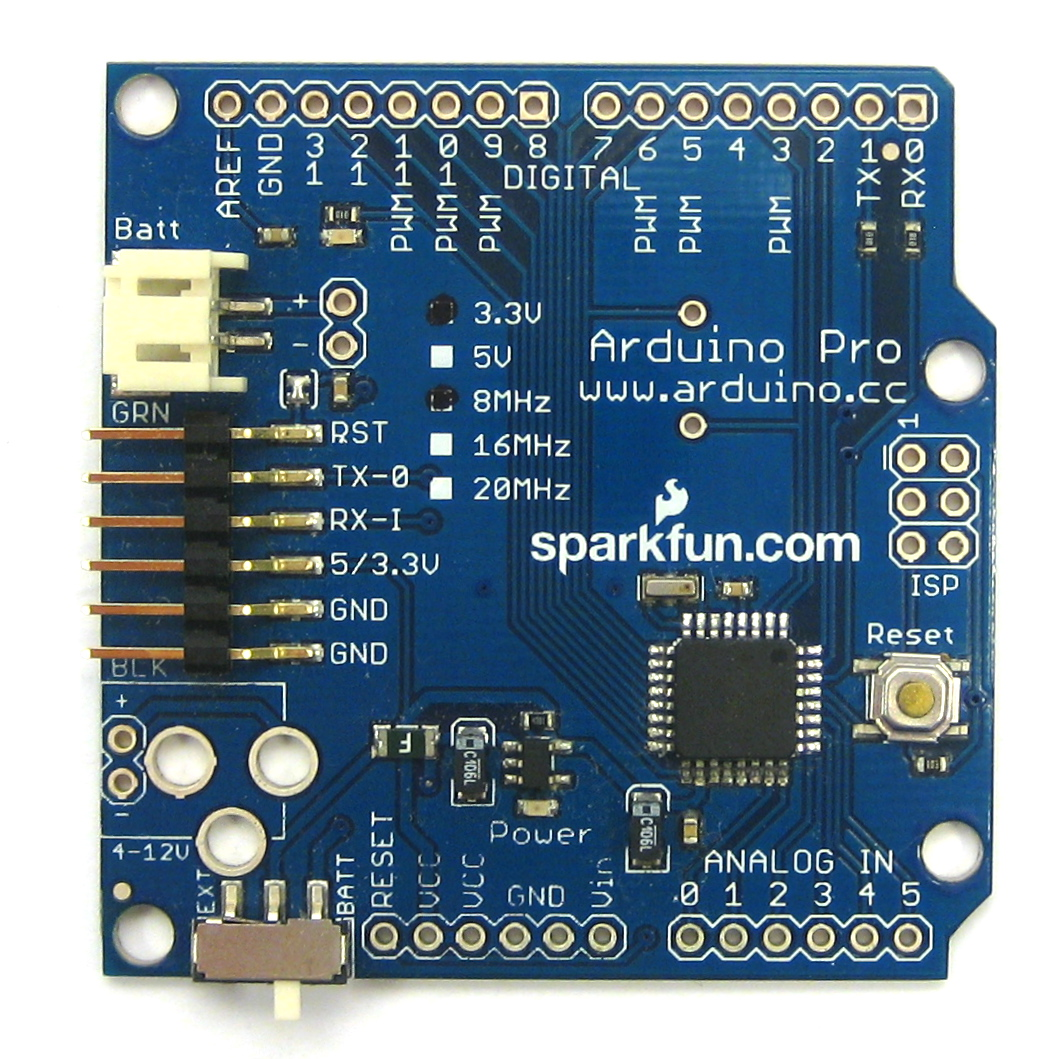
\includegraphics[width=0.8\linewidth]{images/20110115-arduino-pro-print}
    \caption{An Arduino without an FTDI chip.}
    \label{image:no-ftdi-arduino}
  \end{center}
\end{figure}

Note, on the left-hand side, the six pins protruding from the board? If your Arduino requires that you use an FTDI adapter, then you will also need to install drivers. If you aren't 100\% positive, an FTDI adapter tends to look something like this:

\begin{figure}[ht]
  \begin{center}
    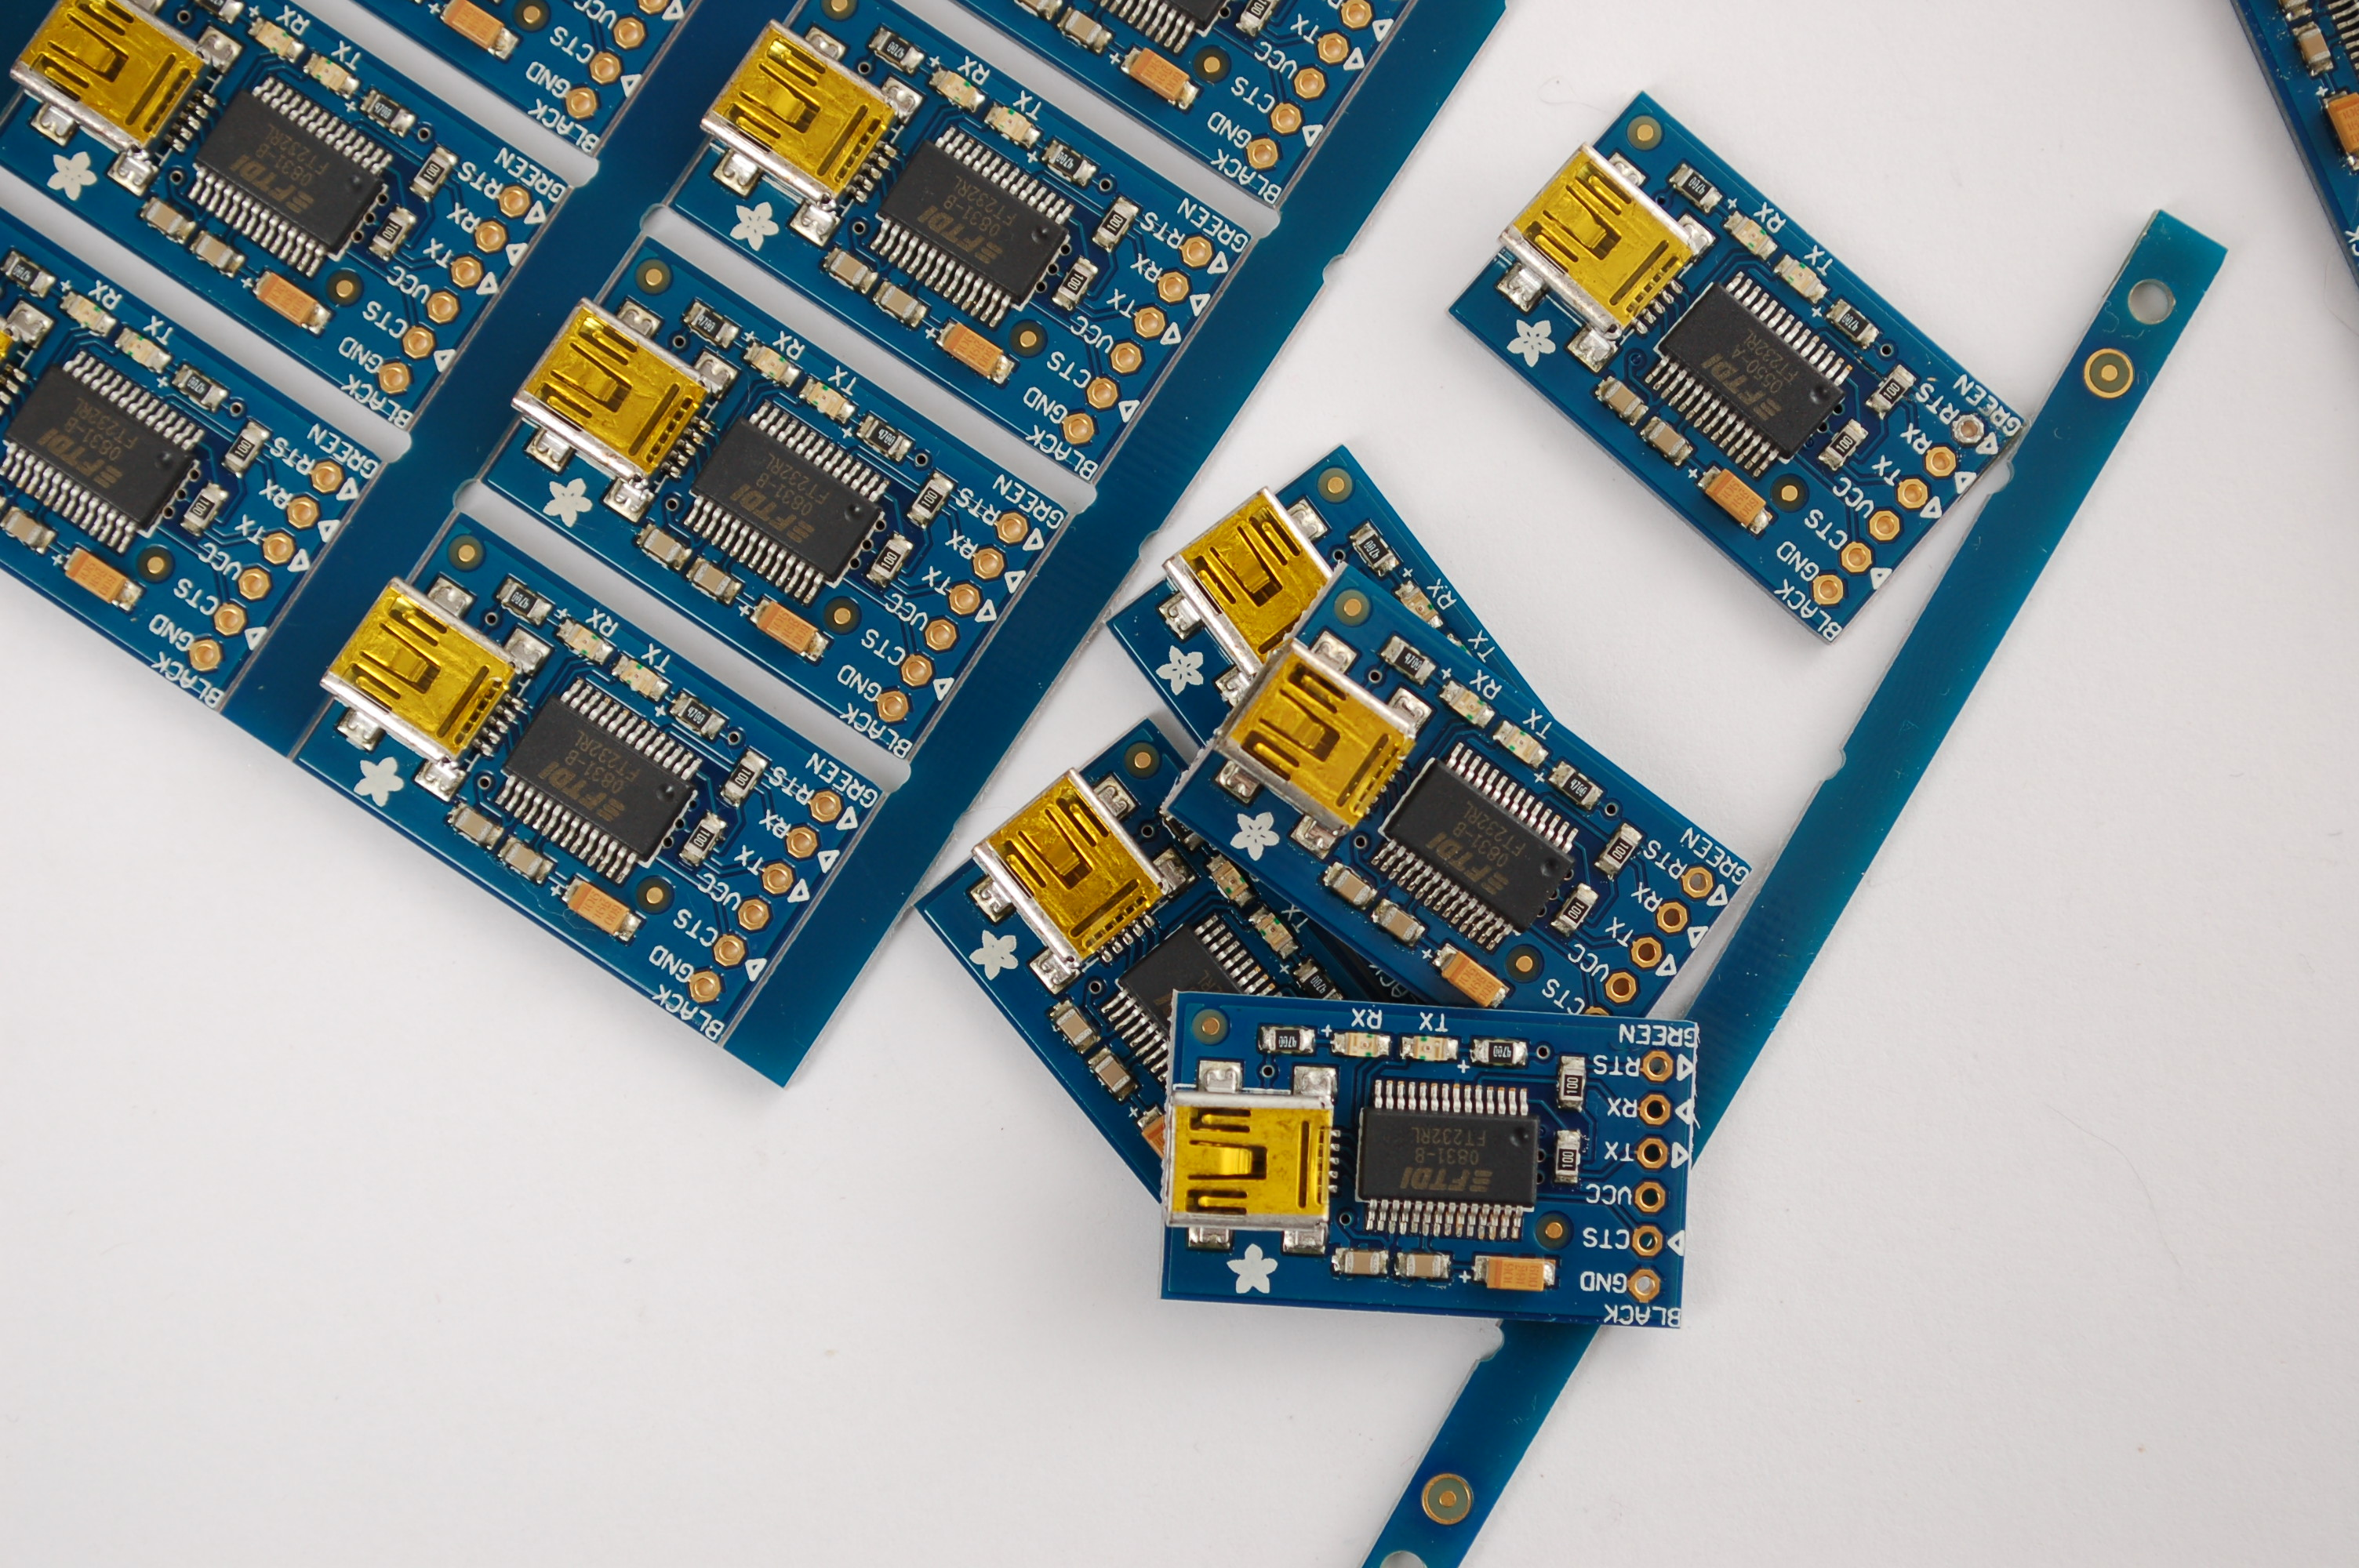
\includegraphics[width=0.8\linewidth]{images/20110115-ftdi-friend-print}
    \caption{The LadyAda {\em FTDI Friend}, an FTDI adapter.}
    \label{image:ftdi-friend}
  \end{center}
\end{figure}

\subsection{You have a new Arduino}
If you have an {\em Arduino Uno} or an {\em Arduino Mega 2560} (the newest Arduinos on the block), you do not need to install anything. You're good to go!

\section{Testing JEdit}
JEdit is a free and open-source editor written in Java. It runs on Mac, Linux, and Windows. We added a ``plug-in'' to this project that lets JEdit talk to your Arduino. You can freely download a version of JEdit from \ccc that has our plug-in pre-configured and ready to go for your choice of operating system.
      
\begin{figure}[!ht]
  \begin{center}
    \includegraphics[height=2.5in]{screenshots/20100108-jedit-docked-occplug}
    \caption{The JEdit program editor.}
    \label{screenshot:jedit-occplug-docked}
  \end{center}
\end{figure}


\subsection{Upload the Firmware}
Before you can run \occam programs on your Arduino, you need to upload some firmware. {\strong Firmware} is code that lives on a processor and executes when it turns on. In the case of \occam programs, we need to install the {\em Transterpreter} on your Arduino---the Transterpreter is the firmware for \occam programs. 

\begin{figure}[!ht]
	\centering
		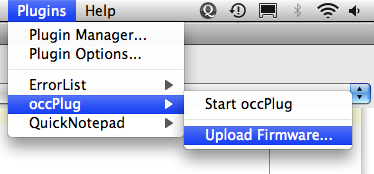
\includegraphics[width=0.6\linewidth]{images/20110115-upload-firmware}
	\caption{Choose ``Upload Firmware'' from the \occplug menu.}
	\label{images:20110115-upload-firmware}
\end{figure}

Selecting this menu option will pop open a window with a set of options like the following:

\begin{figure}[!ht]
	\centering
		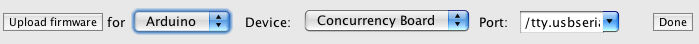
\includegraphics[width=0.9\linewidth]{images/20110115-upload-firmware-window}
	\caption{Select the correct options and upload the firwmare.}
	\label{images:20110115-upload-firmware-window}
\end{figure}

First, select which kind of Arduino you have from the drop-down menu. Then, you need to select your serial port.

\begin{itemize}
	\item On the Mac, the name of the Arduino will look something like {\code /dev/tty.usbserial-A9007U6Z}. 
	\item On Windows, it will be a COM port; you may have to type it in.
	\item On Linux, it should be something like {\code /dev/ttyUSB0}.
\end{itemize}

\newpage

Once you've done that, you can click ``Upload firmware,'' and the Transterpreter will be uploaded to your Arduino. It will then check to see everything was uploaded correctly; it should take around 10 seconds. Once it is done, you can click ``Done,'' and begin writing \occam programs for your Arduino.

\vspace{1cm}
\begin{warning}
The firmware you upload is {\em just an overgrown Arduino sketch}. If you decide to write an Arduino program using Wiring, it will overwrite the \plumbing firmware. So, when you switch back to \occam, the first thing you will have to do is (again) upload the firmware.
\end{warning}
\vspace{1cm}

Put another way, you can freely switch back-and-forth between programs that use \occam and C++, but you have to remember that you need to upload the firmware before an \occam program can be executed.